% trascrizione: Petrillo

\begin{lemma}
	2-numerabile $\implies$ 1-numerabile
\end{lemma}

\begin{proof}
	Sia $\mathcal B$ una base di aperti di $X$ numerabile.
	$\forall x\in X$ sia $\mathcal B_x\is\setdef[A\in\mathcal B]{x\in A}$.
	$\mathcal B_x$ è numerabile ed è una base di intorni di $x$.
\end{proof}

\begin{defn}[Densità]
	Un sottospazio è denso se interseca tutti gli aperti:
	\[\text{$Y$ denso in $X$}\means
	\begin{cases}
		Y\subseteq X\\
		\forall A\text{ aperto},A\neq\nullset:A\cap Y\neq\nullset
	\end{cases}\]
\end{defn}

\begin{lemma}
	\label{th:metrdens2num}
	Uno spazio metrizzabile che contiene un denso numerabile è 2-numerabile:
	\[\begin{rcases}
		X\text{ metrizzabile}\\
		\text{$Y$ denso in $X$ e numerabile}
	\end{rcases}\implies
	X\text{ 2-numerabile}\]
\end{lemma}

\begin{proof}
	\begin{figure}
		\label{fig:binvny}
		\centering
		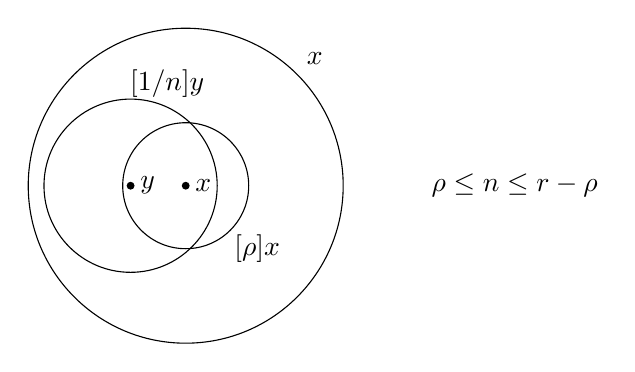
\begin{tikzpicture}
			\coordinate (x) at (0,0);
			\coordinate (y) at (180:0.7);
			\draw (x) node [right] {$x$};
			\fill (x) circle [radius=.05];
			\draw (x) circle [radius=2];
			\draw (x) circle [radius=.8];
			\draw (y) node [right] {$y$};
			\fill (y) circle [radius=.05];
			\draw (y) circle [radius=1.1];
			\draw (x)+(45:2) node [above right] {$\ball x$};
			\draw (x)+(-45:0.7) node [below right] {$\ball[\rho]x$};
			\draw (y)+(65:1.1) node [above] {$\ball[1/n]y$};
			\draw (x)+(0:3) node [right] {$\displaystyle\rho\leq\inv n\leq r-\rho$};
		\end{tikzpicture}
		\caption{Costruzione di $\ball[1/n]y$ tale che $\ball[1/n]y\subseteq\ball x$ e $x\in\ball[1/n]y$.}
	\end{figure}
	Mostriamo che $\setdef[{\ball[1/n]y}]{y\in Y\et n\in\N}$ è una base di aperti di $X$.
	Ogni aperto $A$ si può scrivere come $A=\union_{x\in A}\ball[r_x]x$.
	Scegliamo $\rho_x<r_x$ abbastanza piccolo tale che $\exists n_x\in\N:\rho_x\leq 1/n_x\leq r_x-\rho_x$ (vedi \autoref{fig:binvny}).
	Consideriamo $\ball[\rho_x]x$: è un aperto non vuoto quindi $\exists y_x\in Y\cap\ball[\rho_x]x$.
	Poniamo $A'\is\union_{x\in A}\ball[1/n_x]{y_x}$.
	Allora $A'\subseteq A$ perché $\ball[1/n_x]{y_x}\subseteq\ball[r_x]x$
	e $A\subseteq A'$ perché $x\in\ball[1/n_x]{y_x}$,
	quindi $A=A'$.
\end{proof}

\begin{es}
	$\Q$ è denso in $\R$ e numerabile, quindi $\R$ è 2-numerabile.
	Si noti che nel dimostrare il \autoref{th:metrdens2num} abbiamo usato la densità di $\Q$.
\end{es}

Costruiamo ora una topologia che sia 1-numerabile ma non 2-numerabile:

\begin{defn}
	Sia $\tau_s$ una topologia su $\R$ generata dagli intervalli chiusi a sinistra e aperti a destra:
	\[\tau_s\is\Setdef[\union\mathcal I]{\mathcal I\subseteq\setdef[[a;b)]{a\leq b}}\]
\end{defn}

\begin{prop}
	$\tau_s$ è più fine di $\tau_E$.
\end{prop}

\begin{proof}
	Infatti la topologia euclidea è generata dagli intervalli aperti,
	e ogni intervallo aperto si può scrivere come:
	\[(c;d)=\union_{\substack{a>c\\a<d}}[a;d)
	\qedhere\]
\end{proof}

\begin{prop}
	$\tau_s$ è 1-numerabile.
\end{prop}

\begin{proof}
	Infatti $\Setdef[\left[x;x+\inv n\right)]{n\in\N}$ è una base di intorni di $x$ numerabile.
\end{proof}

\begin{prop}
	$\Q$ è denso in $\R$ secondo $\tau_s$.
\end{prop}

\begin{proof}
	Segue banalmente dalla densità di $\Q$ secondo $\tau_E$.
\end{proof}

\begin{prop}
	$(\R,\tau_s)$ è $T_2$.
\end{prop}

\begin{proof}
	Presi $x<y\,\exists z:x<z<y$ quindi $[x;z)\cap[y;\infty)=\nullset$.
\end{proof}

\begin{prop}
	$(\R,\tau_s)$ non è 2-numerabile
\end{prop}

\begin{proof}
	Sia $\mathcal B$ una base di aperti.
	Abbiamo che:
	\[\forall x\in\R\,\exists B_x\in\mathcal B:
	\begin{cases}
		x\in B_x\\
		B_x\subseteq [x;\infty)
	\end{cases}\]
	Quindi $y\neq x\so B_y\neq B_x$,
	cioè l'applicazione $(x\mapsto B_x)$ da $\R$ in $\mathcal B$ è iniettiva,
	ovvero $\card\mathcal B\geq\card\R$.
\end{proof}

\begin{oss}
	Quindi 1-numerabilità non implica 2-numerabilità.
\end{oss}

Seguono due proposizioni analoghe a quelle mostrate per la proprietà $T_2$:

\begin{prop}
	Le proprietà di numerabilità passano ai sottospazi.
\end{prop}

\begin{prop}
	Le proprietà di numerabilità sono invarianti per omeomorfismo.
\end{prop}

Gli spazi numerabili si possono studiare usando le successioni, cioè le applicazioni con dominio $\N$.
Indichiamo con $(a_n)$ l'applicazione $(n\mapsto a_n)$:

\begin{defn}[Convergenza]
	Si dice che $(a_n)$ \emph{converge a $x$} se è definitivamente contenuta in ogni intorno di $x$:
	\[a_n\convarrow x\means
	\forall U_x\,\exists N\,\forall n\geq N:a_n\in U_x\]
\end{defn}

% gli intorni annidati li ha fatti il 2016-02-22 ma solo per completare questa dimostrazione, quindi li metto qui.
Diamo ora una definizione che ci servirà per dimostrare la \autoref{th:1numaccsucc}:

\begin{defn}
	Una \emph{base di intorni annidati} è una base di intorni numerabile ordinata per inclusione:
	\[\set{U_n}_{n\in\N}\text{ base di intorni annidati}\means
	\begin{cases}
		\set{U_n}\text{base di intorni}\\
		\forall n:U_{n+1}\subseteq U_n
	\end{cases}\]
\end{defn}

\begin{prop}
	Una base di intorni numerabile induce una base di intorni annidati.
\end{prop}

\begin{proof}
	Sia $\set{U_n}_{n\in\N}$ una base di intorni.
	Definiamo $U'_k=\inters_{n=0}^kU_n$.
	$U'_k$~è un intorno perché è un'intersezione finita di intorni.
	$\set{U'_k}_{k\in\N}$ è una base di intorni annidati perché gli $U'_k$ sono tutti contenuti negli $U_n$, e per costruzione sono annidati.
\end{proof}

\begin{prop}
	\label{th:1numaccsucc}
	In uno spazio 1-numerabile, ai punti di accumulazione di un insieme convergono sottosuccessioni a valori nell'insieme:
	\[\begin{rcases}
		X\text{ 1-numerabile }\\
		Y\subseteq X\\
		x\text{ accumulazione per }Y
	\end{rcases}\implies
	\exists(a_n)\subseteq Y:a_n\convarrow x\]
\end{prop}

\begin{proof}
	Sia $\set{U_n}_{n\in\N}$ una base di intorni annidati di $x$.
	Poiché $x$ è di accumulazione per $Y$,
	$\forall n\,\exists a_n\in(U_n\setminus\set x)\cap Y$.
	La successione $(a_n)$ converge a $x$ perché gli $U_n$ sono annidati.
\end{proof}

\titlet{Connessione}

Con la proprietà di connessione vogliamo rendere l'idea intuitiva che uno spazio sia ``tutto attaccato''.

\begin{defn}[Connessione]
	Uno spazio è connesso se non è esprimibile come unione di due aperti disgiunti non vuoti:
	\[X\text{ sconnesso}\means
	\exists A,B\text{ aperti}:
	\begin{cases}
		X=A\cup B\\
		A\cap B=\nullset\\
		A,B\neq\nullset
	\end{cases}\]
\end{defn}

\begin{prop}
	In uno spazio connesso, gli unici insiemi sia aperti che chiusi sono lo spazio stesso e il vuoto:
	\[\begin{rcases}
		X\text{ connesso}\\
		A\subseteq X\\
		A\text{ aperto e chiuso}
	\end{rcases}\implies A=X\vel A=\nullset\]
\end{prop}

\begin{proof}
	$A$ è chiuso quindi $\comp A$ è aperto,
	e $X=A\cup\comp A$.
	Se fosse $A,\comp A\neq\nullset$,
	$X$ sarebbe sconnesso.
\end{proof}

\begin{prop}
	I connessi di $\R$ sono gli intervalli:
	\[Y\subseteq\R\text{ connesso secondo }\tau_E\iff
	Y\text{ è un intervallo}\]
\end{prop}

\begin{proof}
	Mostriamo le due implicazioni:
	\begin{description}
		\item[\proofrightarrow]
			Se $Y$ non fosse un intervallo, avremmo
			$\exists x\in(\inf Y;\sup Y):x\not\in Y$.
			Ma allora $Y=\big(Y\cap(-\infty;x)\big)\cup\big(Y\cap(x;\infty)\big)\absurd$.
		\item[\proofleftarrow]
			Supponiamo per assurdo che $Y$ sia sconnesso.
			Allora $Y=A_1\cup A_2$ aperti (nella topologia di $Y$) disgiunti non vuoti.
			In particolare $\exists x_1\in A_1,x_2\in A_2\wlg x_1<x_2$.
			Poiché $Y$ è un intervallo, $[x_1;x_2]\subseteq Y$.
			Poniamo:
			\[\xi\is\sup(A_1\cap[x_1;x_2])=\min(x_2,\sup A_1)\]
			$\xi$ è di accumulazione per $A_1$ e $A_2$, quindi
			$\xi\in\clos{A_1}\cap\clos{A_2}$.
			Ma essendo gli $A_i$ complementari in $Y$, $A_i=\clos{A_i}\absurd$.
			\qedhere
	\end{description}
\end{proof}
